% Options for packages loaded elsewhere
\PassOptionsToPackage{unicode}{hyperref}
\PassOptionsToPackage{hyphens}{url}
\PassOptionsToPackage{dvipsnames,svgnames,x11names}{xcolor}
%
\documentclass[
  12pt,
]{article}
\usepackage{amsmath,amssymb}
\usepackage{lmodern}
\usepackage{iftex}
\ifPDFTeX
  \usepackage[T1]{fontenc}
  \usepackage[utf8]{inputenc}
  \usepackage{textcomp} % provide euro and other symbols
\else % if luatex or xetex
  \usepackage{unicode-math}
  \defaultfontfeatures{Scale=MatchLowercase}
  \defaultfontfeatures[\rmfamily]{Ligatures=TeX,Scale=1}
\fi
% Use upquote if available, for straight quotes in verbatim environments
\IfFileExists{upquote.sty}{\usepackage{upquote}}{}
\IfFileExists{microtype.sty}{% use microtype if available
  \usepackage[]{microtype}
  \UseMicrotypeSet[protrusion]{basicmath} % disable protrusion for tt fonts
}{}
\makeatletter
\@ifundefined{KOMAClassName}{% if non-KOMA class
  \IfFileExists{parskip.sty}{%
    \usepackage{parskip}
  }{% else
    \setlength{\parindent}{0pt}
    \setlength{\parskip}{6pt plus 2pt minus 1pt}}
}{% if KOMA class
  \KOMAoptions{parskip=half}}
\makeatother
\usepackage{xcolor}
\usepackage[margin=1in]{geometry}
\usepackage{color}
\usepackage{fancyvrb}
\newcommand{\VerbBar}{|}
\newcommand{\VERB}{\Verb[commandchars=\\\{\}]}
\DefineVerbatimEnvironment{Highlighting}{Verbatim}{commandchars=\\\{\}}
% Add ',fontsize=\small' for more characters per line
\usepackage{framed}
\definecolor{shadecolor}{RGB}{248,248,248}
\newenvironment{Shaded}{\begin{snugshade}}{\end{snugshade}}
\newcommand{\AlertTok}[1]{\textcolor[rgb]{0.94,0.16,0.16}{#1}}
\newcommand{\AnnotationTok}[1]{\textcolor[rgb]{0.56,0.35,0.01}{\textbf{\textit{#1}}}}
\newcommand{\AttributeTok}[1]{\textcolor[rgb]{0.77,0.63,0.00}{#1}}
\newcommand{\BaseNTok}[1]{\textcolor[rgb]{0.00,0.00,0.81}{#1}}
\newcommand{\BuiltInTok}[1]{#1}
\newcommand{\CharTok}[1]{\textcolor[rgb]{0.31,0.60,0.02}{#1}}
\newcommand{\CommentTok}[1]{\textcolor[rgb]{0.56,0.35,0.01}{\textit{#1}}}
\newcommand{\CommentVarTok}[1]{\textcolor[rgb]{0.56,0.35,0.01}{\textbf{\textit{#1}}}}
\newcommand{\ConstantTok}[1]{\textcolor[rgb]{0.00,0.00,0.00}{#1}}
\newcommand{\ControlFlowTok}[1]{\textcolor[rgb]{0.13,0.29,0.53}{\textbf{#1}}}
\newcommand{\DataTypeTok}[1]{\textcolor[rgb]{0.13,0.29,0.53}{#1}}
\newcommand{\DecValTok}[1]{\textcolor[rgb]{0.00,0.00,0.81}{#1}}
\newcommand{\DocumentationTok}[1]{\textcolor[rgb]{0.56,0.35,0.01}{\textbf{\textit{#1}}}}
\newcommand{\ErrorTok}[1]{\textcolor[rgb]{0.64,0.00,0.00}{\textbf{#1}}}
\newcommand{\ExtensionTok}[1]{#1}
\newcommand{\FloatTok}[1]{\textcolor[rgb]{0.00,0.00,0.81}{#1}}
\newcommand{\FunctionTok}[1]{\textcolor[rgb]{0.00,0.00,0.00}{#1}}
\newcommand{\ImportTok}[1]{#1}
\newcommand{\InformationTok}[1]{\textcolor[rgb]{0.56,0.35,0.01}{\textbf{\textit{#1}}}}
\newcommand{\KeywordTok}[1]{\textcolor[rgb]{0.13,0.29,0.53}{\textbf{#1}}}
\newcommand{\NormalTok}[1]{#1}
\newcommand{\OperatorTok}[1]{\textcolor[rgb]{0.81,0.36,0.00}{\textbf{#1}}}
\newcommand{\OtherTok}[1]{\textcolor[rgb]{0.56,0.35,0.01}{#1}}
\newcommand{\PreprocessorTok}[1]{\textcolor[rgb]{0.56,0.35,0.01}{\textit{#1}}}
\newcommand{\RegionMarkerTok}[1]{#1}
\newcommand{\SpecialCharTok}[1]{\textcolor[rgb]{0.00,0.00,0.00}{#1}}
\newcommand{\SpecialStringTok}[1]{\textcolor[rgb]{0.31,0.60,0.02}{#1}}
\newcommand{\StringTok}[1]{\textcolor[rgb]{0.31,0.60,0.02}{#1}}
\newcommand{\VariableTok}[1]{\textcolor[rgb]{0.00,0.00,0.00}{#1}}
\newcommand{\VerbatimStringTok}[1]{\textcolor[rgb]{0.31,0.60,0.02}{#1}}
\newcommand{\WarningTok}[1]{\textcolor[rgb]{0.56,0.35,0.01}{\textbf{\textit{#1}}}}
\usepackage{longtable,booktabs,array}
\usepackage{calc} % for calculating minipage widths
% Correct order of tables after \paragraph or \subparagraph
\usepackage{etoolbox}
\makeatletter
\patchcmd\longtable{\par}{\if@noskipsec\mbox{}\fi\par}{}{}
\makeatother
% Allow footnotes in longtable head/foot
\IfFileExists{footnotehyper.sty}{\usepackage{footnotehyper}}{\usepackage{footnote}}
\makesavenoteenv{longtable}
\usepackage{graphicx}
\makeatletter
\def\maxwidth{\ifdim\Gin@nat@width>\linewidth\linewidth\else\Gin@nat@width\fi}
\def\maxheight{\ifdim\Gin@nat@height>\textheight\textheight\else\Gin@nat@height\fi}
\makeatother
% Scale images if necessary, so that they will not overflow the page
% margins by default, and it is still possible to overwrite the defaults
% using explicit options in \includegraphics[width, height, ...]{}
\setkeys{Gin}{width=\maxwidth,height=\maxheight,keepaspectratio}
% Set default figure placement to htbp
\makeatletter
\def\fps@figure{htbp}
\makeatother
\setlength{\emergencystretch}{3em} % prevent overfull lines
\providecommand{\tightlist}{%
  \setlength{\itemsep}{0pt}\setlength{\parskip}{0pt}}
\setcounter{secnumdepth}{5}
\newlength{\cslhangindent}
\setlength{\cslhangindent}{1.5em}
\newlength{\csllabelwidth}
\setlength{\csllabelwidth}{3em}
\newlength{\cslentryspacingunit} % times entry-spacing
\setlength{\cslentryspacingunit}{\parskip}
\newenvironment{CSLReferences}[2] % #1 hanging-ident, #2 entry spacing
 {% don't indent paragraphs
  \setlength{\parindent}{0pt}
  % turn on hanging indent if param 1 is 1
  \ifodd #1
  \let\oldpar\par
  \def\par{\hangindent=\cslhangindent\oldpar}
  \fi
  % set entry spacing
  \setlength{\parskip}{#2\cslentryspacingunit}
 }%
 {}
\usepackage{calc}
\newcommand{\CSLBlock}[1]{#1\hfill\break}
\newcommand{\CSLLeftMargin}[1]{\parbox[t]{\csllabelwidth}{#1}}
\newcommand{\CSLRightInline}[1]{\parbox[t]{\linewidth - \csllabelwidth}{#1}\break}
\newcommand{\CSLIndent}[1]{\hspace{\cslhangindent}#1}
\usepackage{setspace}\doublespacing
\ifLuaTeX
  \usepackage{selnolig}  % disable illegal ligatures
\fi
\IfFileExists{bookmark.sty}{\usepackage{bookmark}}{\usepackage{hyperref}}
\IfFileExists{xurl.sty}{\usepackage{xurl}}{} % add URL line breaks if available
\urlstyle{same} % disable monospaced font for URLs
\hypersetup{
  pdftitle={Description of the project to be submitted},
  pdfauthor={Stephan.Huber@hs-fresenius.de},
  colorlinks=true,
  linkcolor={red},
  filecolor={Maroon},
  citecolor={Blue},
  urlcolor={blue},
  pdfcreator={LaTeX via pandoc}}

\title{Description of the project to be submitted}
\author{\href{mailto:Stephan.Huber@hs-fresenius.de}{\nolinkurl{Stephan.Huber@hs-fresenius.de}}}
\date{Last compiled on 06 June, 2023}

\begin{document}
\maketitle
\begin{abstract}
In the following I describe the project that needs to be submitted in the course \emph{Data Science for Business}. I give some hints for your efficient progress and success, I introduce the elements and files to be submitted, and I describe how I evaluate the submissions.
\end{abstract}

{
\hypersetup{linkcolor=}
\setcounter{tocdepth}{3}
\tableofcontents
}
\hypertarget{main-goal}{%
\section{Main goal}\label{main-goal}}

\textbf{Course description}
\emph{`'Students complete this module with a project work. The project work includes a project report (15-20 pages) and a project presentation (20-30 minutes).''}

\textbf{Project work}

\begin{itemize}
\tightlist
\item
  Find an interesting academic research paper that provides the dataset that are necessary to replicate the results shown in the paper,
\item
  replicate the results shown in the paper using R,
\item
  write a report of your work in progress, and
\item
  present your current status of the project in class.
\end{itemize}

\hypertarget{details}{%
\section{Details}\label{details}}

\begin{itemize}
\tightlist
\item
  Choose your paper wisely. It should be a compelling read for you, and you should have a basic understanding of the research methods applied. Papers can vary greatly in complexity, length, and methodological level.
\item
  You don't need to replicate the entire paper. Replicating a single table, specific columns, or a single visualization can be sufficient. The goal is to document your progress and to demonstrate your proficiency in using R as a tool to work with data.
\item
  Reflect on both your successes and failures, as well as any challenges you encountered. For instance, if a line of code took a significant amount of time to write, you can explain the issue to me, but keep it concise.
\item
  I highly recommend that you discuss the paper you want to replicate with me and ask for supervision. This will help ensure that you are on the right track and have the support you need.
\item
  I kindly request that you come to me rather than waiting for me to come to you. This will help facilitate our communication and ensure that we are both on the same page.
\end{itemize}

\hypertarget{the-report}{%
\subsection{The report}\label{the-report}}

The report should aim to be around 5000-6000 words, or approximately 15 double-spaced pages. Please note that this report is different from an academic paper in that it should focus solely on documenting, discussing, and presenting your project. Its purpose is to introduce your work to me in a way that is similar to reports written in business settings, where you would need to convey what you did, why you did it that way, what obstacles you overcame, what challenges, problems and weaknesses remain, and how you would suggest proceeding with your work if you had more time and resources.

Please refrain from trying to impress me with a fancy layout or any extraneous details. Your primary focus should be on effectively communicating your current state of work to the reader. Feel free to include anything that can help achieve this goal.

Please put some emphasize on guiding and motivating the reader. For example, the introduction is a good place to introduce the scope and content of the report.

To ensure conciseness and clarity, please eliminate all unnecessary repetition. Take the time to read each sentence multiple times and ask yourself if it is concise, clear, and coherent with what was said before and after.

Finally, please use R Markdown to write your report. You can use the .Rmd file included with this document as a template. This file is hosted at \href{https://github.com/hubchev/courses/tree/main/rmd}{my GitHub page:} Information about writing and publishing with R Markdown can be found here:

\begin{itemize}
\tightlist
\item
  \href{https://rmarkdown.rstudio.com/lesson-1.html}{R Markdown from R Studio}
\item
  \href{https://bookdown.org/yihui/rmarkdown/}{R Markdown: The Definitive Guide} written by Xie, Allaire, \& Grolemund (2018).
\item
  \href{https://bookdown.org/yihui/rmarkdown-cookbook/}{R Markdown Cookbook} written by Xie, Dervieux, \& Riederer (2020).
\end{itemize}

Insert R code in your R markdown file by typing the chunk delimiters (see the keyboard shortcut \emph{Ctrl+Alt+I} for Windows and Linux based OS and \emph{Cmd+Option+I} for Macintosh OS) or \href{https://rmarkdown.rstudio.com/lesson-3.html}{this lesson}).

The outline of the paper \textbf{must} contain the following building blocks:

\begin{itemize}
\tightlist
\item
  Title and all common personal details (name, email, \ldots).
\item
  Word count (see below on how to give a word count).
\item
  Abstract of the paper (which highlights the content of the document).
\item
  All the R code that is necessary to replicate your results.
\end{itemize}

\hypertarget{the-presentation}{%
\subsection{The presentation}\label{the-presentation}}

\begin{itemize}
\tightlist
\item
  Write the presentation using R Markdown and publish it as .html and/or a .pdf file.
\item
  Focus on the important things.
\item
  Try to stay on time.
\item
  Nobody is perfect and the project is done under time pressure. So don't try to sell yourself too hard. If you see weaknesses in your work, this is a good place to discuss them.
\item
  Describe and present your paper and the data set used in it.
\item
  To facilitate the organization and scheduling of all presentations, please let me know the times you are available by \textbf{April 22}. A maximum of 3 presentations per meeting would be ideal. If you do not let me know your preferences, I will determine the time and date. Here is the link where you can give me your preferences and your availability:
  \href{https://doodle.com/meeting/participate/id/bojvq6Ya}{Doodle Poll: Data Science Presentation}
\end{itemize}

\hypertarget{rmd-file}{%
\subsection{rmd file}\label{rmd-file}}

\begin{itemize}
\tightlist
\item
  The rmd file should contain the complete workflow including data import, data cleaning, and data analysis.
\item
  All code but not all the output generated by the code should be shown in the pdf paper. See \href{https://rmarkdown.rstudio.com/lesson-3.html}{Code Chunks and R Markdown} how to set certain options to prevent code and results from appearing in the finished file.
\end{itemize}

\hypertarget{affidavit}{%
\subsection{Affidavit}\label{affidavit}}

\emph{Your report should contain the following \textbf{Affidavit}. Simply, fill it out and put it at the end of your report. You can check the box like this:}

\begin{itemize}
\tightlist
\item[$\boxtimes$]
  I checked this box
\end{itemize}

\begin{center}\rule{0.5\linewidth}{0.5pt}\end{center}

I hereby affirm that this submitted paper was authored unaided and
solely by me. Additionally, no other sources than those in the reference
list were used. Parts of this paper, including tables and figures, that
have been taken either verbatim or analogously from other works have in
each case been properly cited with regard to their origin and
authorship. This paper either in parts or in its entirety, be it in the
same or similar form, has not been submitted to any other examination
board and has not been published.

I have read the Handbook of Academic Writing by Hildebrandt \& Nelke (2019) and
have endeavored to comply with the guidelines and standards set forth
therein.

I acknowledge that the university may use plagiarism detection software
to check my thesis. I agree to cooperate with any investigation of
suspected plagiarism and to provide any additional information or
evidence requested by the university.

I assure the project report contains the following:

\begin{itemize}
\tightlist
\item[$\square$]
  The report is written in R Markdown.
\end{itemize}

The report contains\ldots{}

\begin{itemize}
\item[$\square$]
  \ldots{} 5000-6000 words.
\item[$\square$]
  \ldots{} a title and personal detail (name, email, matriculation
  number).
\item[$\square$]
  \ldots{} a word count.
\item[$\square$]
  \ldots{} an abstract.
\item[$\square$]
  \ldots{} a bibliography that was created using BibTeX applying an APA
  citation style.
\item[$\square$]
  \ldots{} the complete R code that is necessary to replicate your
  results.
\item[$\square$]
  \ldots{} detailed information on how the data are downloaded and read
  in to R.
\item[$\square$]
  \ldots{} an introduction where you guide the reader and a conclusion
  where you summarize your work and discuss what you would work on if
  you would have more time available.
\item[$\square$]
  \ldots{} all significant resources that were used to write the report
  and the R code.
\item[$\square$]
  \ldots{} the filled out \emph{Affidavit}.
\item[$\square$]
  \ldots a brief description of the successful contribution using Git and GitHub as explained here: \url{https://github.com/hubchev/ds_summer23}.
\end{itemize}

The submission of the project contains\ldots{}

\begin{itemize}
\tightlist
\item[$\square$]
  \ldots{} the .Rmd file of the
  report.
\item[$\square$]
  \ldots{} the .pdf file of the report.
\item[$\square$]
  \ldots{} the .html file of the report.
\item[$\square$]
  \ldots{} all files necessary that are not available online to reproduce the report and the R code therein.
\item[$\square$]
  \ldots{} the .Rmd file of the presentation.
\item[$\square$]
  \ldots{} the .html file of the presentation.
\end{itemize}

{[}Your Name,{]} {[}Date,{]} {[}Place{]}

\begin{center}\rule{0.5\linewidth}{0.5pt}\end{center}

\hypertarget{submission}{%
\section{Submission}\label{submission}}

\begin{itemize}
\tightlist
\item
  Submission deadline for academic papers and written assessments: \textbf{24 July 2023} \emph{(please verify!)}
\item
  Upload only \textbf{one .zip file} containing the following:

  \begin{enumerate}
  \def\labelenumi{\arabic{enumi}.}
  \tightlist
  \item
    the paper as (a) .pdf and a (b) .html file.
  \item
    the .Rmd file
  \item
    the data set (if not too large),
  \item
    the presentation as (a) .Rmd and a (b) .html file,
  \item
    additional files, if needed, so that I can evaluate your work.
  \end{enumerate}
\item
  Please also submit to my Github account at \url{https://github.com/hubchev/ds_summer23} and mention that in the report.
\end{itemize}

\hypertarget{evaluation}{%
\section{Evaluation}\label{evaluation}}

\begin{itemize}
\item
  \emph{65 \% -- Quality and execution of the project}
  -- After your presentation, we will discuss your work in a personal meeting. The goal of this conversation will be that we agree on certain standards by which I will grade you. By this I mean that we define certain goals that you should achieve with your data set and your question. The goal is to create a transparent set of expectations on my part. So that you have an indication of what you need to accomplish at a minimum in order to pass the course.
\item
  \emph{35 \% -- Quality and execution of the presentation}
\item
  I will try to evaluate your work as objectively as possible. In particular, I will

  \begin{itemize}
  \tightlist
  \item
    check whether your submission is complete, or not,
  \item
    check whether your empirical work can be reproduced,
  \item
    check if all formal criteria are met,
  \item
    check for plagiarism,
  \item
    check if the replication of the paper was already done with R by somebody else,
  \item
    read your work and evaluate your writing skills (clarity, coherence, grammar, etc.),
  \item
    review and evaluate the difficulty level of your project,
  \item
    evaluate the technical level of use of the programming language R for your empirical goals,
  \item
    assess whether your empirical reasoning makes sense and discuss your remaining weaknesses,
  \item
    acknowledge your learning process.
  \end{itemize}
\end{itemize}

\hypertarget{helpful-stuff}{%
\section{Helpful stuff}\label{helpful-stuff}}

\hypertarget{r-markdown}{%
\subsection{R Markdown}\label{r-markdown}}

To knit to all formats that are mentioned in the header, type that into the console (of course, don't forget to refer to your working directory using setwd()):

\begin{Shaded}
\begin{Highlighting}[]
\FunctionTok{setwd}\NormalTok{(}\StringTok{"/home/sthu/Dropbox/hsf/github/courses/rmd/"}\NormalTok{)}
\NormalTok{rmarkdown}\SpecialCharTok{::}\FunctionTok{render}\NormalTok{(}\StringTok{"23{-}04\_ds{-}project{-}desc.Rmd"}\NormalTok{, }\StringTok{"all"}\NormalTok{)}
\end{Highlighting}
\end{Shaded}

\hypertarget{git-and-github}{%
\subsection{Git and GitHub}\label{git-and-github}}

As you should submit your work to my Github account, you can learn how to do that by following the instructions of this repository: \url{https://github.com/hubchev/ds_summer23}

\hypertarget{word-count}{%
\subsection{Word count}\label{word-count}}

You can include a word count in various ways. Here are two alternatives:

This code installs and loads the required packages and save the words counted:

\begin{Shaded}
\begin{Highlighting}[]
\CommentTok{\#install.packages("devtools")}
\CommentTok{\#library("devtools")}
\CommentTok{\#devtools::install\_github("benmarwick/wordcountaddin", type = "source", dependencies = T)}
\FunctionTok{library}\NormalTok{(}\StringTok{"wordcountaddin"}\NormalTok{)}
\NormalTok{wordcount }\OtherTok{\textless{}{-}}\NormalTok{ wordcountaddin}\SpecialCharTok{::}\FunctionTok{word\_count}\NormalTok{( )}
\end{Highlighting}
\end{Shaded}

\textbf{Word count:} 1650

Word count (alternative): 1906

\hypertarget{include-figures-and-tables}{%
\subsection{Include figures and tables}\label{include-figures-and-tables}}

There are different ways to include figures and tables. I do not recommend doing it with html code as this does not work with pdf output. In figure \ref{fig:itsme} and \ref{fig:figofme} you see two identical pictures of me but two different ways to include pics.

\begin{figure}
\centering
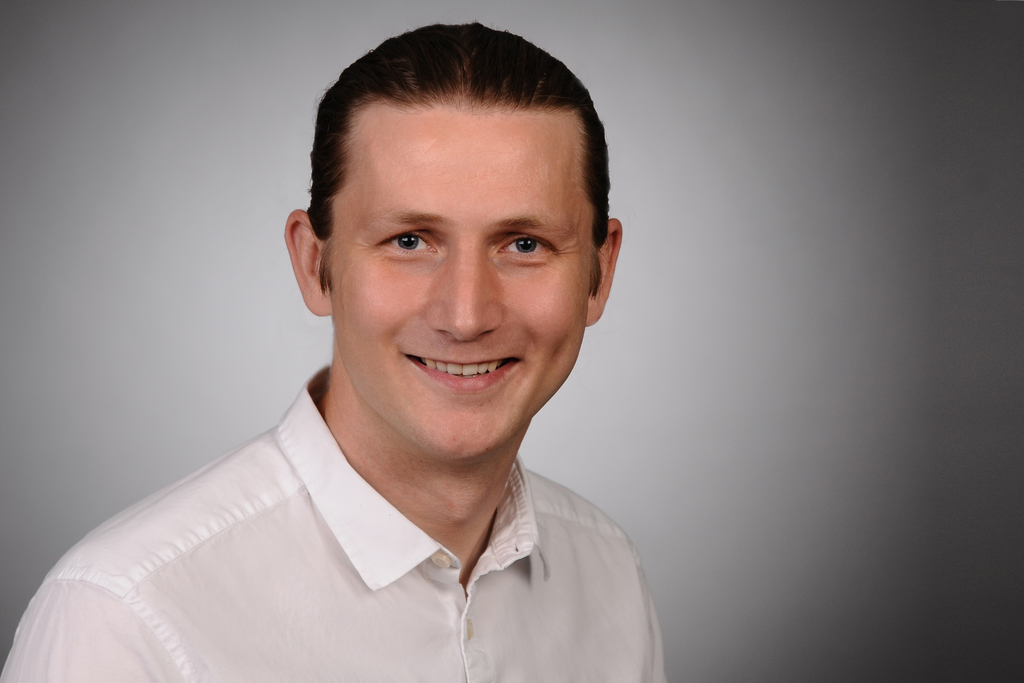
\includegraphics[width=0.25\textwidth,height=\textheight]{../pic/huber2.jpeg}
\caption[\label{fig:itsme} Prof.~Dr.~Stephan Huber]{\label{fig:itsme} Prof.~Dr.~Stephan Huber\footnotemark{}}
\end{figure}
\footnotetext{Picture is taken from \url{https://sites.google.com/view/stephanhuber}}

\begin{figure}

{\centering 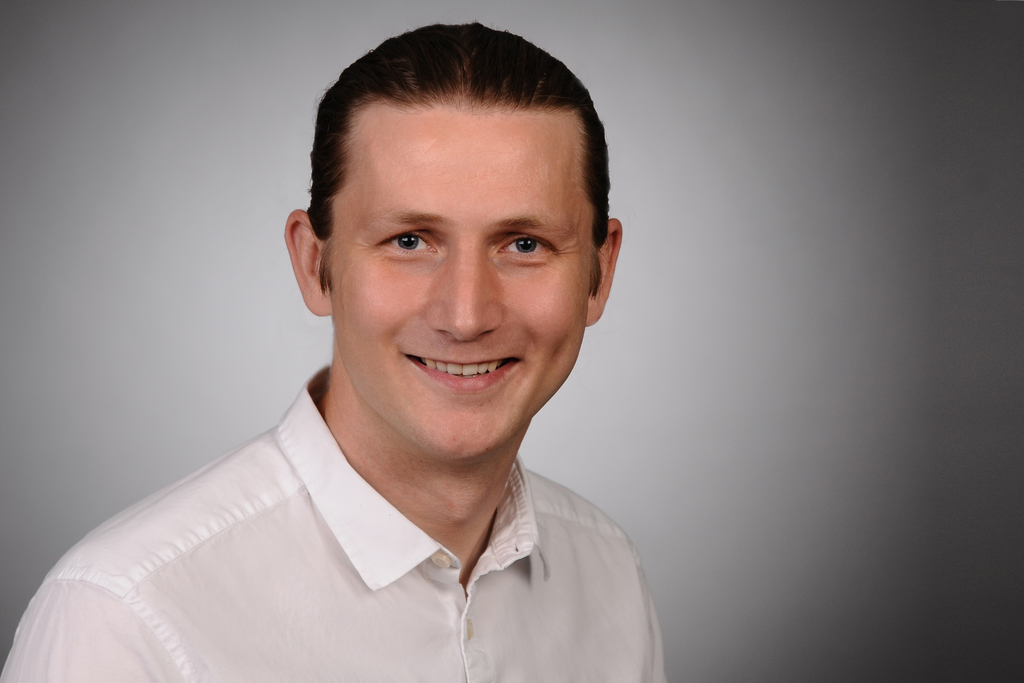
\includegraphics[width=0.2\linewidth]{../pic/huber2} 

}

\caption{Prof. Dr. Stephan Huber}\label{fig:figofme}
\end{figure}

\hypertarget{literature}{%
\section*{Literature}\label{literature}}
\addcontentsline{toc}{section}{Literature}

\hypertarget{refs}{}
\begin{CSLReferences}{1}{0}
\leavevmode\vadjust pre{\hypertarget{ref-Hildebrandt2019Handbook}{}}%
Hildebrandt, J., \& Nelke, M. (Eds.). (2019). \emph{Handbook of academic writings}. Bonn, Germany: VNR Verlag f{ü}r die Deutsche Wirtschaft.

\leavevmode\vadjust pre{\hypertarget{ref-Xie2018R}{}}%
Xie, Y., Allaire, J. J., \& Grolemund, G. (2018). \emph{R markdown: The definitive guide}. Retrieved January 30, 2023; Chapman; Hall/CRC. Retrieved from \url{https://bookdown.org/yihui/rmarkdown/}

\leavevmode\vadjust pre{\hypertarget{ref-Xie2020R}{}}%
Xie, Y., Dervieux, C., \& Riederer, E. (2020). \emph{R markdown cookbook}. Retrieved January 30, 2023; Chapman; Hall/CRC. Retrieved from \url{https://bookdown.org/yihui/rmarkdown-cookbook}

\end{CSLReferences}

\end{document}
